\documentclass{beamer}
\usepackage{ulem}
\usepackage{tikz}
\usepackage{booktabs}
 \usepackage{graphicx,threeparttable,caption}
\usetikzlibrary{shapes,snakes}
\usepackage[beamer,customcolors]{hf-tikz}
\usepackage{nicematrix}
\usepackage{xcolor}
\usepackage{makecell}
\usepackage{array}
\usepackage{csquotes}
\usepackage{csquotes}
\usepackage{minted}
\captionsetup{labelformat=empty,labelsep=none}

\graphicspath{ {./png/} }
\tikzset{hl/.style={
    set fill color=red!80!black!40,
    set border color=red!80!black,
  },
}
\AtBeginSection[]{
  \begin{frame}
  \vfill
  \centering
  \begin{beamercolorbox}[sep=8pt,center,shadow=true,rounded=true]{title}
    \usebeamerfont{title}\insertsectionhead\par%
  \end{beamercolorbox}
  \vfill
  \end{frame}
}
%\usecolortheme[orchid]{structure}
\usetheme[hideothersubsections]{PaloAlto}
\makeatletter
\patchcmd{\csq@bquote@i}{{#6}}{{\emph{#6}}}{}{}
\makeatother
%\usecolortheme{orchid}
%\usefonttheme{professionalfonts}
\newcommand{\soutthick}[1]{%
   \textcolor{red}{
   \renewcommand{\ULthickness}{1pt}%
      \sout{#1}%
   \renewcommand{\ULthickness}{.4pt}% Resetting to ulem default
   }
}
\newcommand{\centered}[1]{\begin{tabular}{l} #1 \end{tabular}}
\setbeamertemplate{section in toc}[square]
\setbeamertemplate{subsection in toc}[square]
\setbeamertemplate{secion in sidebar}[shaded]
\setbeamertemplate{items}[square]
\setbeamercovered{transparent} 

\title[]{Programming in Python for Social Scientists}
\subtitle{Introduction}
\author[]{Mikołaj Biesaga\\ \small{\color{blue}{\href{mailto:m.biesaga@uw.edu.pl}{m.biesaga@uw.edu.pl}}}}
\institute{
\includegraphics[width = 4 cm]{uw.png}}
\date{\today}
\begin{document}
\begin{frame}
   \titlepage
\end{frame}

\begin{frame}
    \frametitle{Mikołaj Biesaga}
    \only<+>{
        \framesubtitle{Best Book Ever}
        \begin{center}
            
\includegraphics[width = .4\textwidth]{gww.jpg}
        \end{center}
    }
    \only<+>{
        \framesubtitle{Current Book}
        \begin{center}
            
\includegraphics[width = .4\textwidth]{strange_beasts.jpg}
        \end{center}
    }
    \only<+>{
        \framesubtitle{Current Series}
        \begin{center}
            
\includegraphics[width = .5\textwidth]{severance.jpg}
        \end{center}
    }
\end{frame}

\section{Rules of Engagement}

\begin{frame}
    \frametitle{Office Hours, Emails, Presentations, etc.}
    \begin{description}[Google Classroom:]
        \item [Office Hours:] write me an email before coming
        \item [Emails:] the official info will go through emails
        \item [GitHub:] scripts (notebooks) will be posted on GitHub
        \item [Google Classroom:] materials and presentations will be posted on
        Google Classroom
    \end{description}
    \alert{I will try to answer your inquiries as soon as possible but do not
    count on an immediate response, especially right before the deadlines.}
\end{frame}
\begin{frame}
    \frametitle{Emails}
        
\includegraphics[width = \textwidth]{emails.png}
\end{frame}
\begin{frame}
    \frametitle{Workflow}
    \begin{enumerate}
        \item Presentation of the basic concepts in the classroom
        \item Exercises in the classroom
        \item [<3] Homework assignments requiring modifying the work done in the classroom
    \end{enumerate}
\end{frame}
\begin{frame}
    \frametitle{Assessment Criteria}
    \begin{itemize}
        \item The final grade will be determined based on \alert{5 homework
        assignments}
        \item The first 4 homework (after classes: 2, 3, 4, and 5) will be scored from 0 to 10 points and the
        last one (after the last class) from 0 to 20 points.
        \item Grading criteria:
    \begin{description}
        \item [5\phantom{+} --] => 54 points
        \item [4+ --] 51 - 53 points
        \item [4\phantom{+} --] 45 - 50 points
        \item [3+ --] 42 - 44 points
        \item [3\phantom{+} --] 36 - 41 points
        \item [2\phantom{+} --] =< 35 points
    \end{description}
\end{itemize}
\end{frame}
\begin{frame}
    \frametitle{Attendance}
    \only<1>{
        \begin{itemize}
            \item Attendance is \alert{obligatory}
            \item You are allowed to miss up to \alert{2 classes in case of a formal
            excuse}
            \item An absence does not exempt from doing homework assignments
        \end{itemize}
    }
    \only<2>{
        \begin{center}
            
\includegraphics[width = .9\textwidth]{png/pretty_please.jpg}
        \end{center}
    }
\end{frame}

\begin{frame}
    \frametitle{Additional Resources}
    \only<1>{
        \begin{center}
            \includegraphics<1>[width = .5\textwidth]{copy_paste.png}
        \end{center}
    }
    \only<2>{
        \begin{center}
            \includegraphics<2>[width = .6\textwidth]{stack_overflow.png}
        \end{center}
    }
    \only<3>{
        \begin{itemize}
            \item \textcolor{blue}{\href{https://stackoverflow.com}{www.stackoverflow.com}}
            \item \textcolor{blue}{\href{https://www.learnpython.org}{www.learnpython.org}}
            \item \textcolor{blue}{\href{https://www.edx.org/course/introduction-to-computer-science-and-programming-7?index=product&queryID=51a933646c74acd8353b1d8c34fa59d6&position=2}{Introduction to Computer Science and Programming Using Python}}
            \item Introduction to Computation and Programming Using Python by John V. Guttag
        \end{itemize}
    }
    \only<4>{
        \begin{center}
            \includegraphics<4>[width=\textwidth]{chatgpt_stackoverflow.png}
        \end{center}
    }
    \only<5>{
        \begin{center}
            \includegraphics<5>[width=\textwidth]{chatgpt.png}
        \end{center}
    }
    \only<6>{
        \begin{center}
            \includegraphics<6>[width = \textwidth]{chatgpt_meme_original.jpg}
        \end{center}
    }
    \only<7>{
        \begin{center}
            \includegraphics<7>[width=.5\textwidth]{chatgpt_meme.jpg}
        \end{center}
    }
    \only<8>{
        \begin{center}
            \includegraphics<8>[width=.7\textwidth]{chatgpt2025.png}
        \end{center}
    }
    
\end{frame}

\section{How Social Scientists can use Python?}

\begin{frame}
    \only<+>{
        \centering
        
\includegraphics[width = \framewidth]{png/python_logo.png}
    }
    \only<2,3>{
        \frametitle{What is Python?}
        \only<2>{
            \begin{definition}
                \emph{Pythons} are a family of nonvenomous snakes found in Africa, Asia, and Australia. Among its members are some of the largest snakes in the world. Ten genera and 42 species are currently recognized.
            \end{definition}
        }
        \only<3>{
            \begin{definition}
                \emph{Python} is a programming language and the Python interpreter is a piece of software that reads the source code and performs its instructions. There are two generations of Python: Python 2.x and Python 3.x. \alert{We will use Python 3.x only.}
            \end{definition}
        }
    }
    \only<4>{
        \frametitle{Python}
        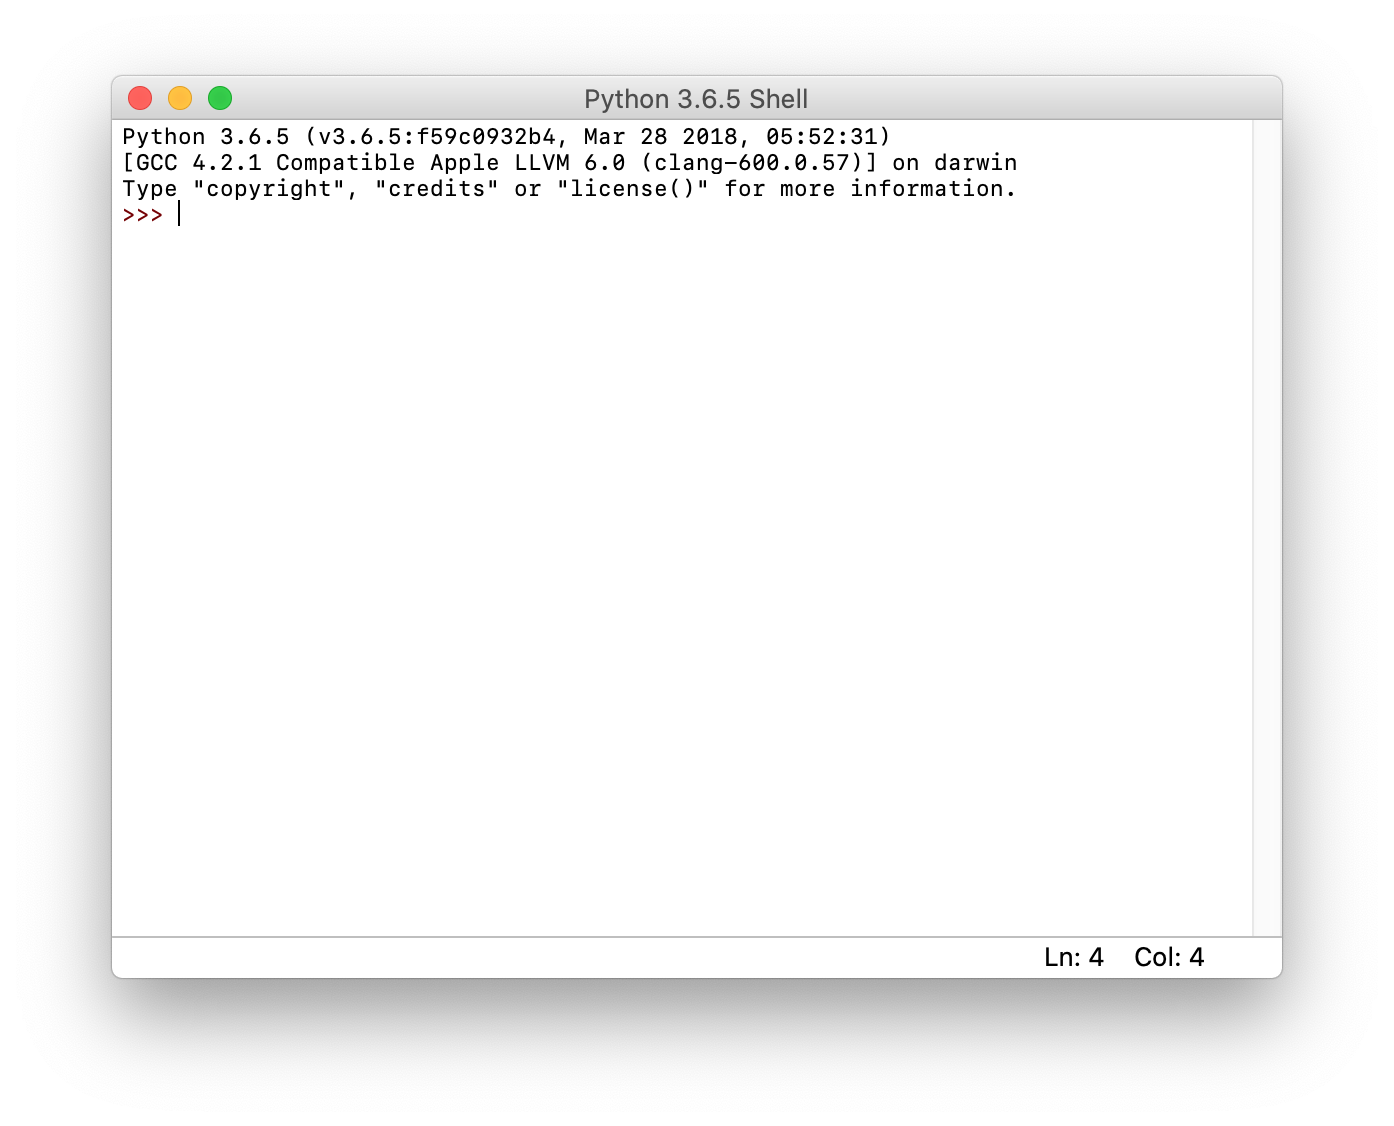
\includegraphics[width = \framewidth]{png/python_idle.png}
    }
\end{frame}

\begin{frame}
    \frametitle{How Social Scientists can use Python?}
    \only<1,3,5,7,9,11>{
        \begin{itemize}
            \item<1> extraction of unstructured data from external digital (i.e. web-based) sources
            \item<3> analysis of textual data (natural language processing -- NLP)
            \item<5> designing experiments
            \item<7> working with big datasets 
            \item<9> network and relational data analysis
            \item<11> computer simulations
        \end{itemize}
    }
    \only<2>{
        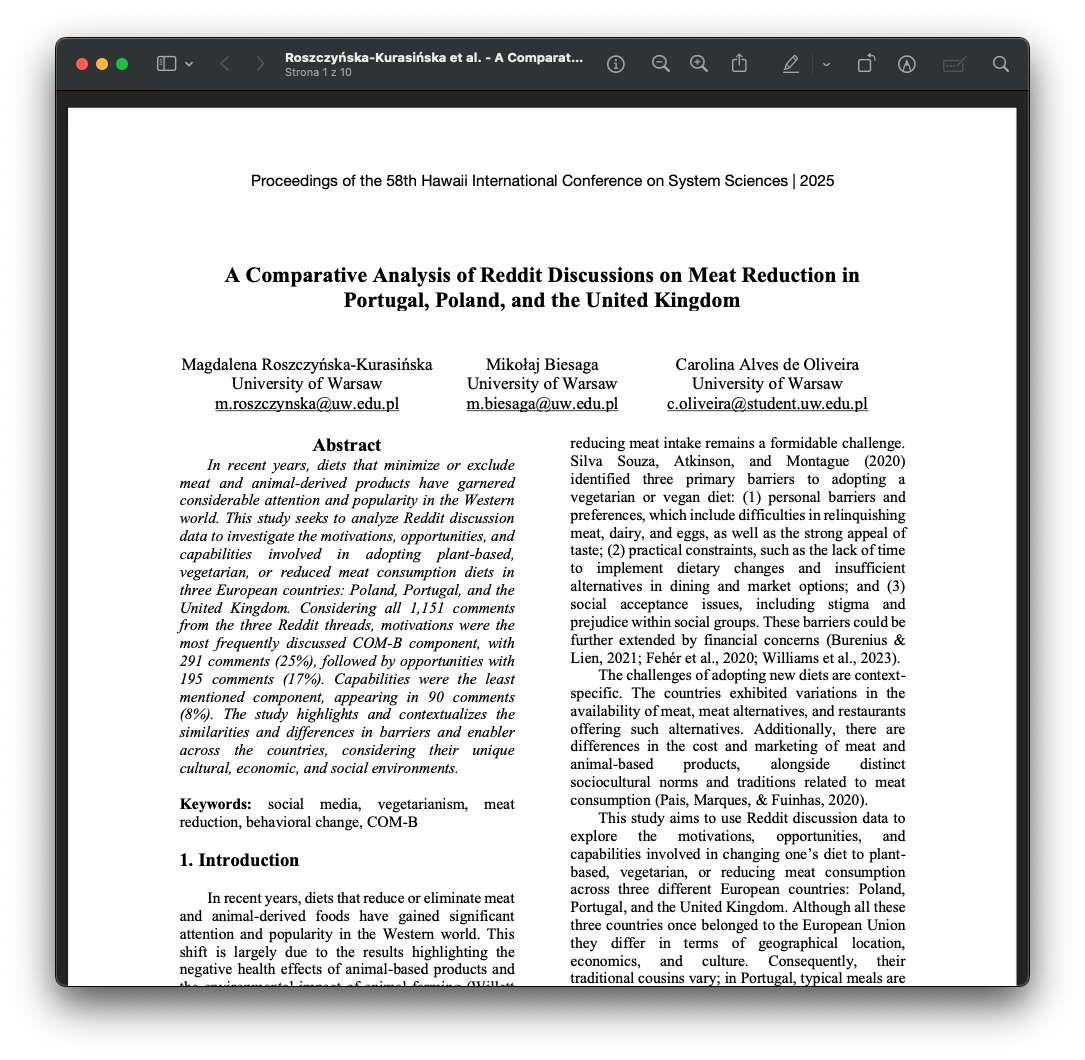
\includegraphics[width = \textwidth]{carolina.png}
    }
    \only<4>{
        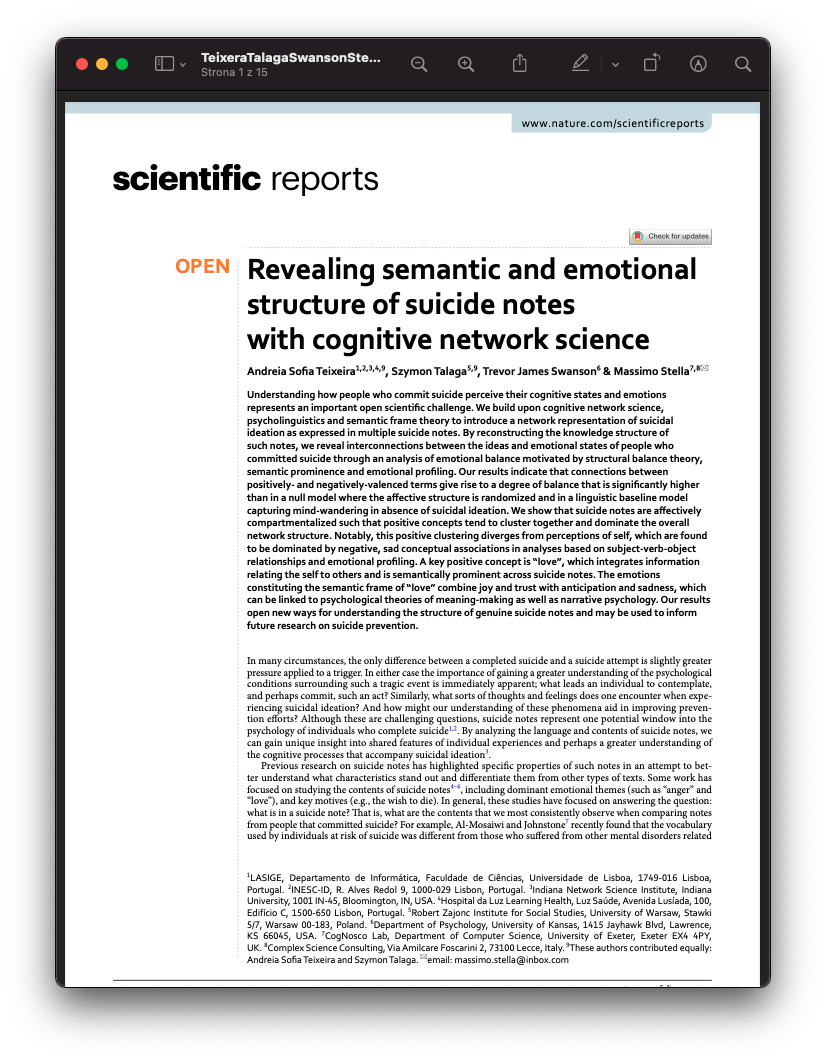
\includegraphics[width = \textwidth]{nlp.png}
    }
    \only<6>{
        
\includegraphics[width = \textwidth]{designing.png}
    }
    \only<8>{
        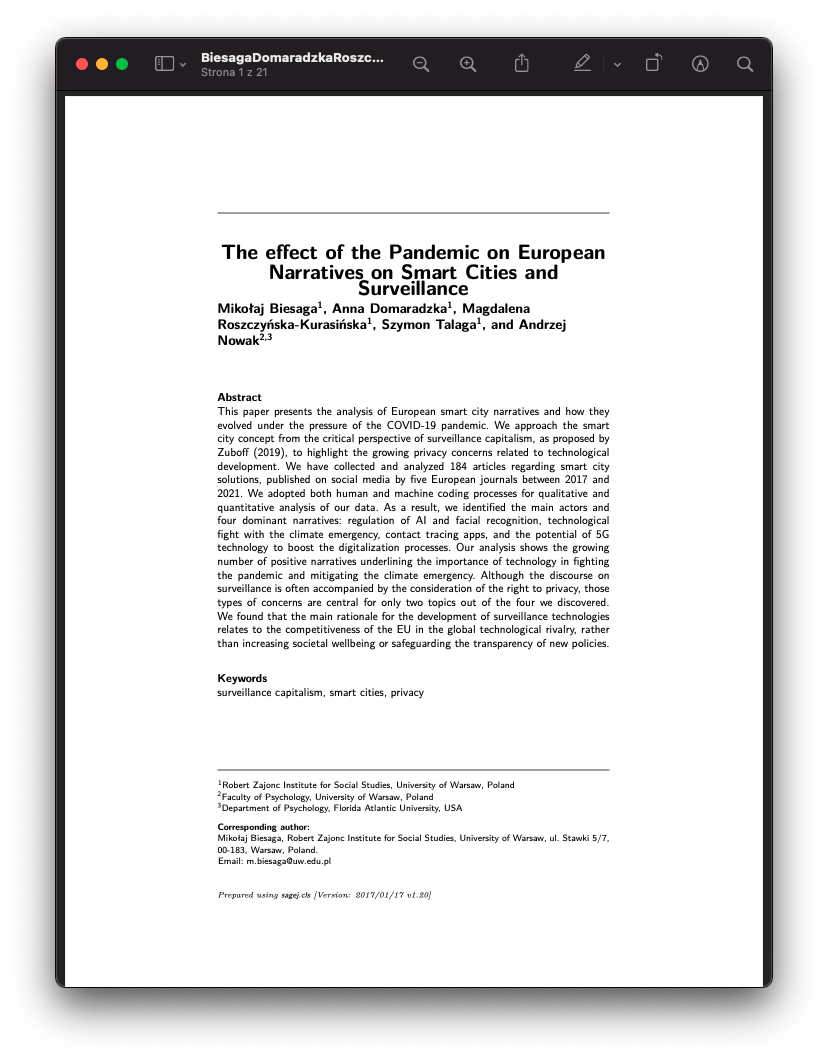
\includegraphics[width = \textwidth]{big_data.png}
    }
    \only<10>{
        
\includegraphics[width = \textwidth]{networks.png}
    }
    \only<12>{
        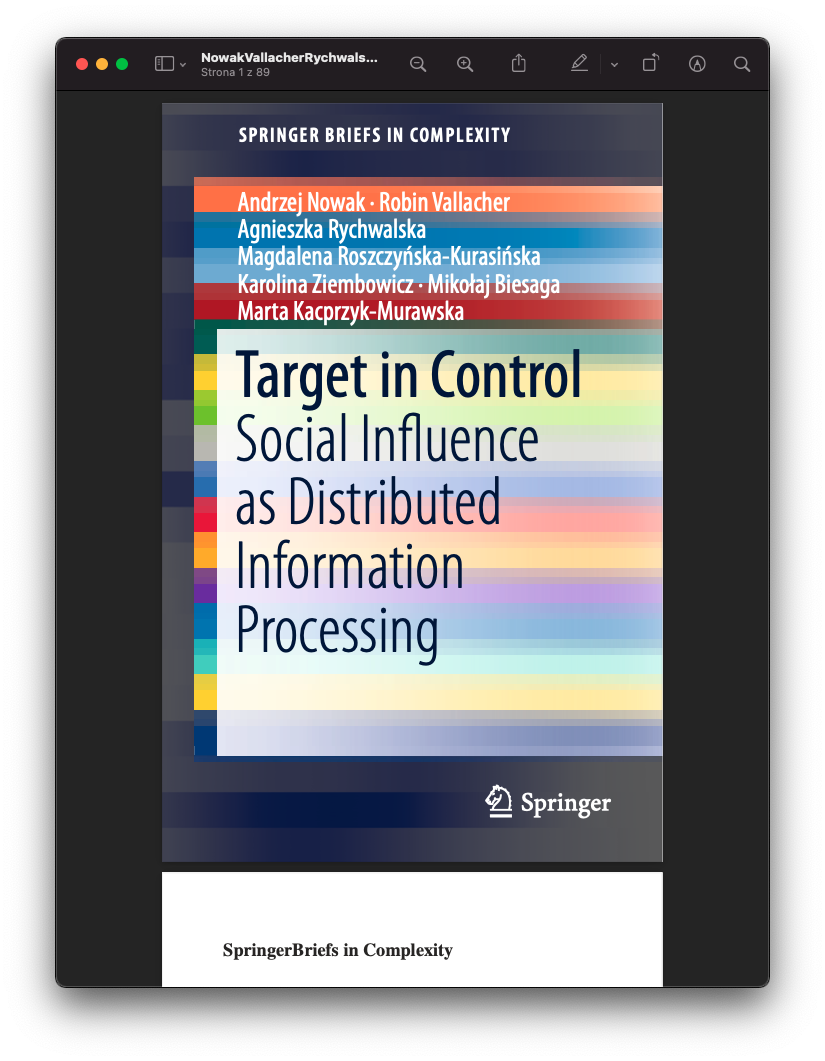
\includegraphics[width = \textwidth]{simulations.png}
    }

\end{frame}

\section{Objectives}

\begin{frame}
    \frametitle{Objective of the course}
    \begin{itemize}
        \item present basic programming concepts in Python
        \item present how Social Scientists can use programming languages
        \item present where to find resources and solutions to basic computing problems
        \item teach you how to solve basic computing problems with the use of Python
        \item teach you the importance of writing readable and reproducible code
    \end{itemize}
    \only<2>{
        \alert{You will not be a Computer Scientist after the course!}
    }
\end{frame}

\section{Tools of the trade}

\begin{frame}
    \only<+>{
        \centering
        
\includegraphics[width = .6\framewidth]{png/jupyter.png}
    }
    \only<+>{
        \frametitle{What is Jupyter Notebook?}
        \begin{definition}
            \emph{Jupyter Notebooks} are documents produced by the Jupyter Notebook App which contain both computer code (e.g. python) and rich text elements (paragraph, equations, figures, links, etc.). Notebook documents are both human-readable documents containing the analysis description and the results (figures, tables, etc.) as well as executable documents that can be run to perform data analysis.
        \end{definition}
    }
    \only<+>{
        \frametitle{Jupyter Notebook}
        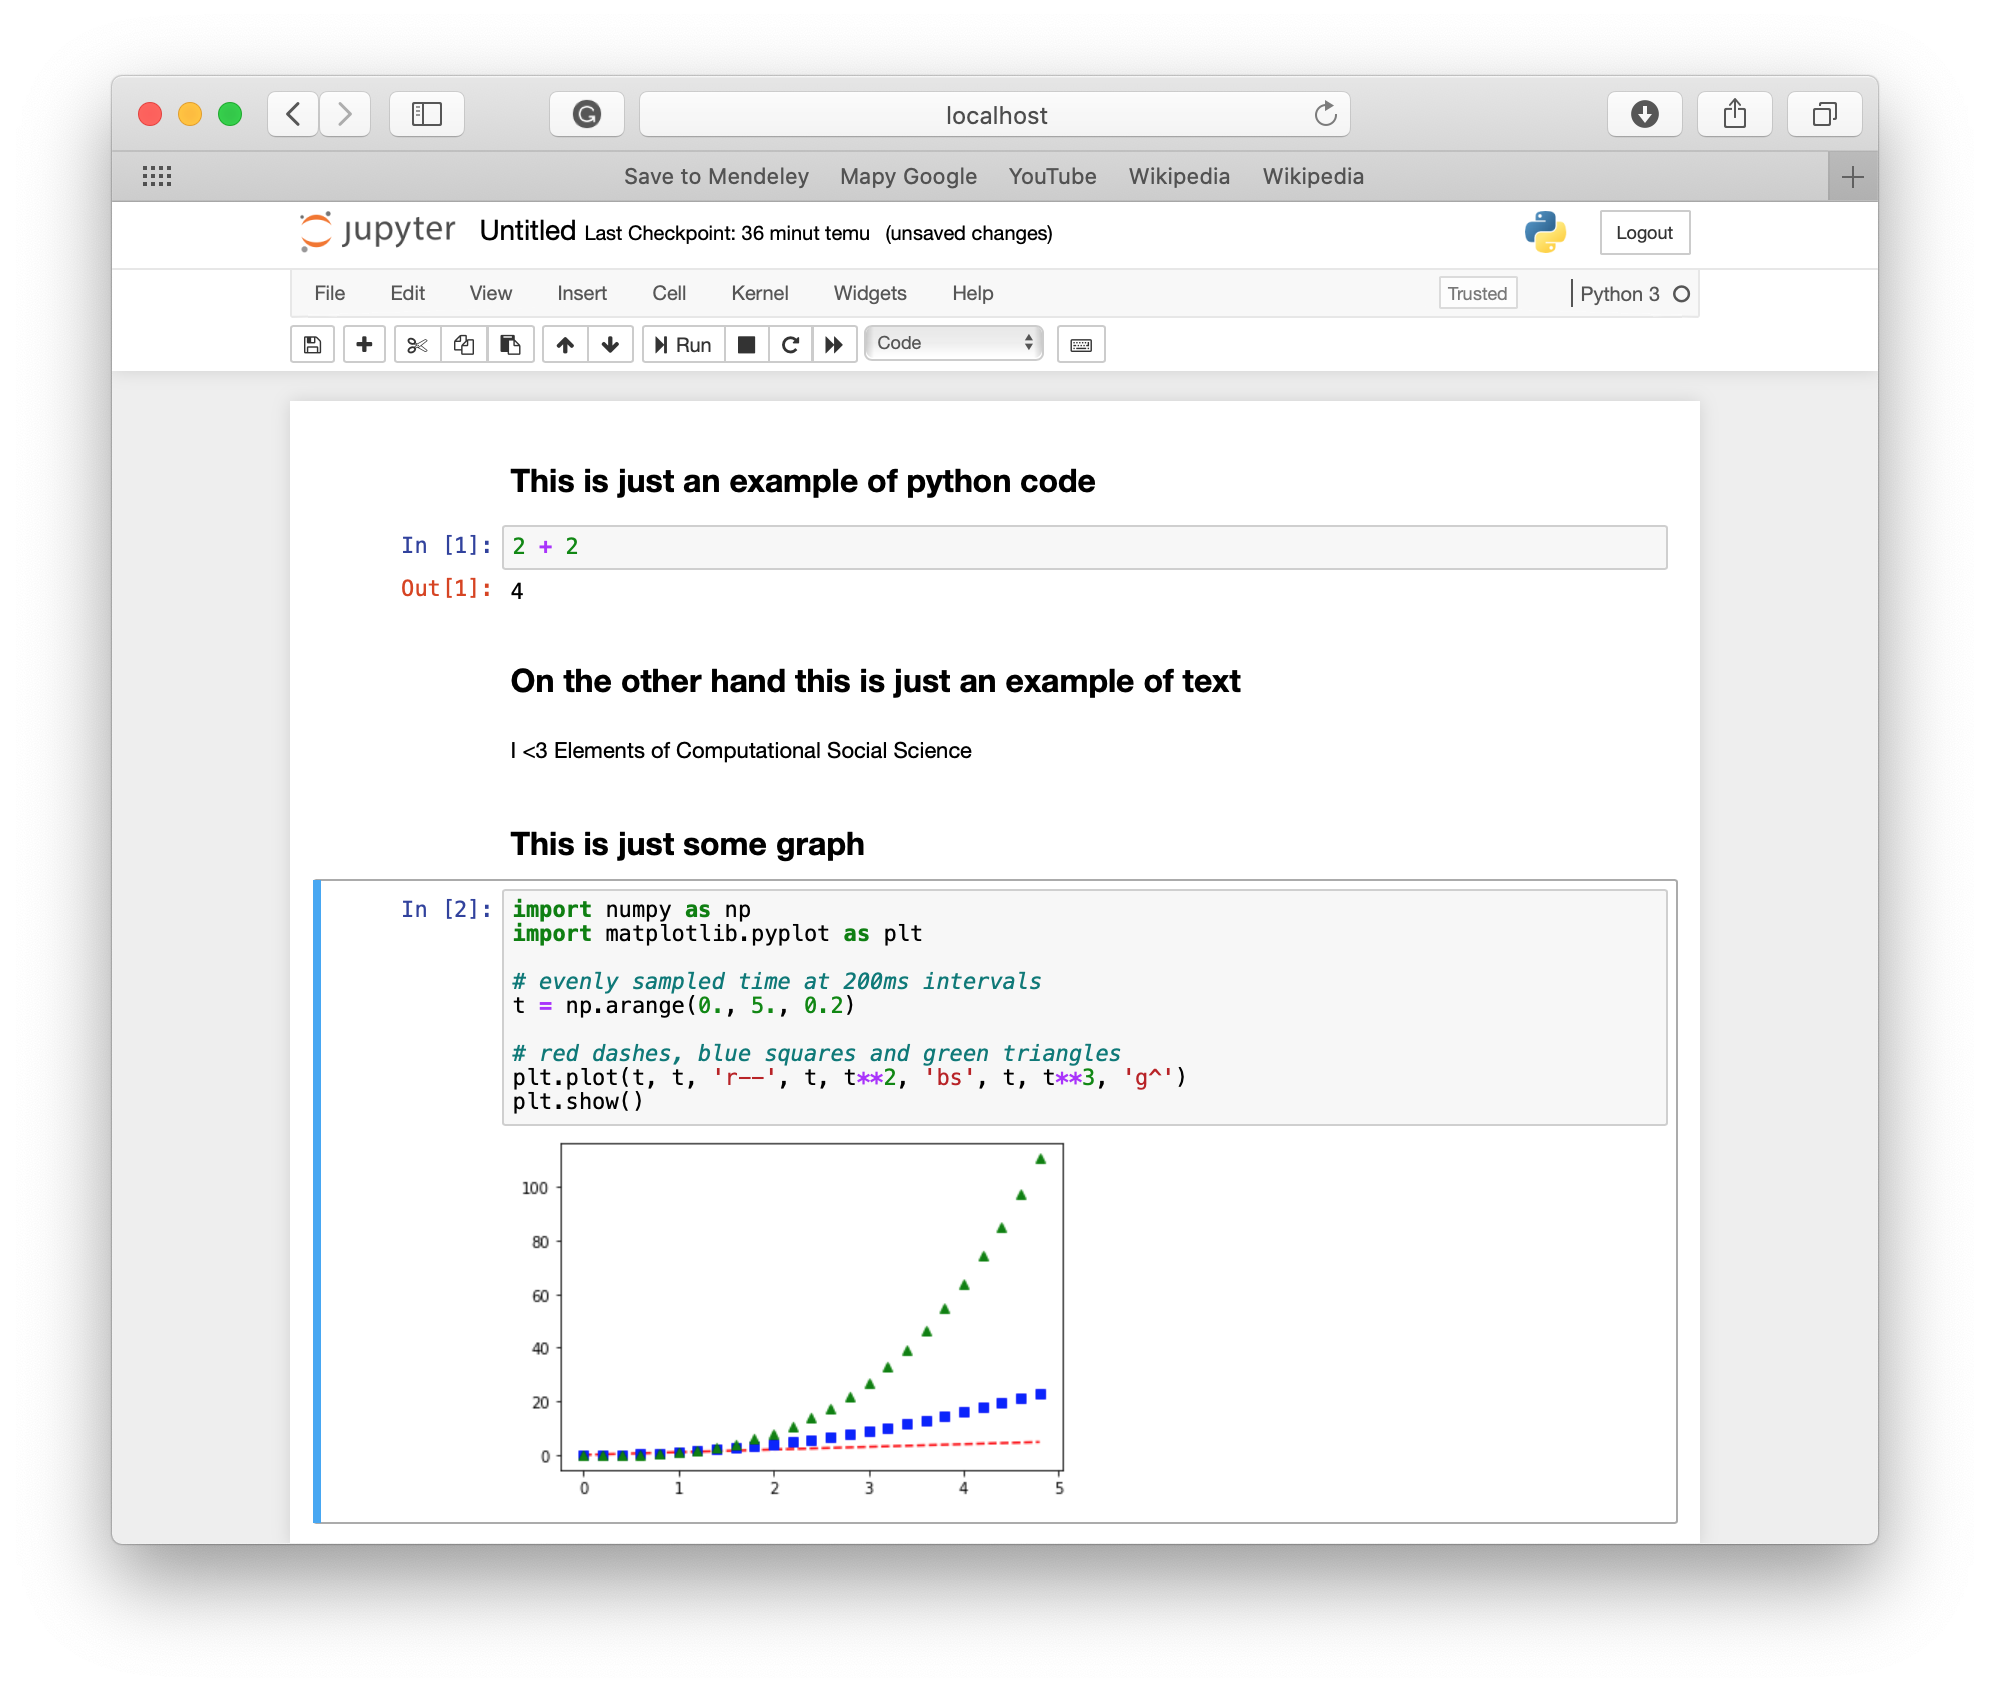
\includegraphics[width = \framewidth]{png/jupyter_notebook.png}
    }
    \only<+>{
        \frametitle{What is Jupyter Notebook App?}
        \begin{definition}
            \emph{The Jupyter Notebook App} is an application that allows editing and running code via a web browser. The app can be run on a local desktop requiring no internet access or can be installed on a remote server and accessed through the internet.
        \end{definition}
    }
\end{frame}

\begin{frame}[fragile]
    \only<+>{
        \begin{center}
            
\includegraphics[scale = .7]{png/colab.png}
        \end{center}
    }
    \only<+>{
        \frametitle{What is Colaboratory?}
        \begin{definition}
            \emph{Colaboratory} is a free Jupyter Notebook environment that requires no setup and runs entirely in the cloud. In other words, it is almost the same as Jupyter Notebook App but it runs in Google Cloud, so if you have a google account you have access to Colaboratory.
        \end{definition}
    }
    \only<+>{
        \frametitle{Colaboratory}
        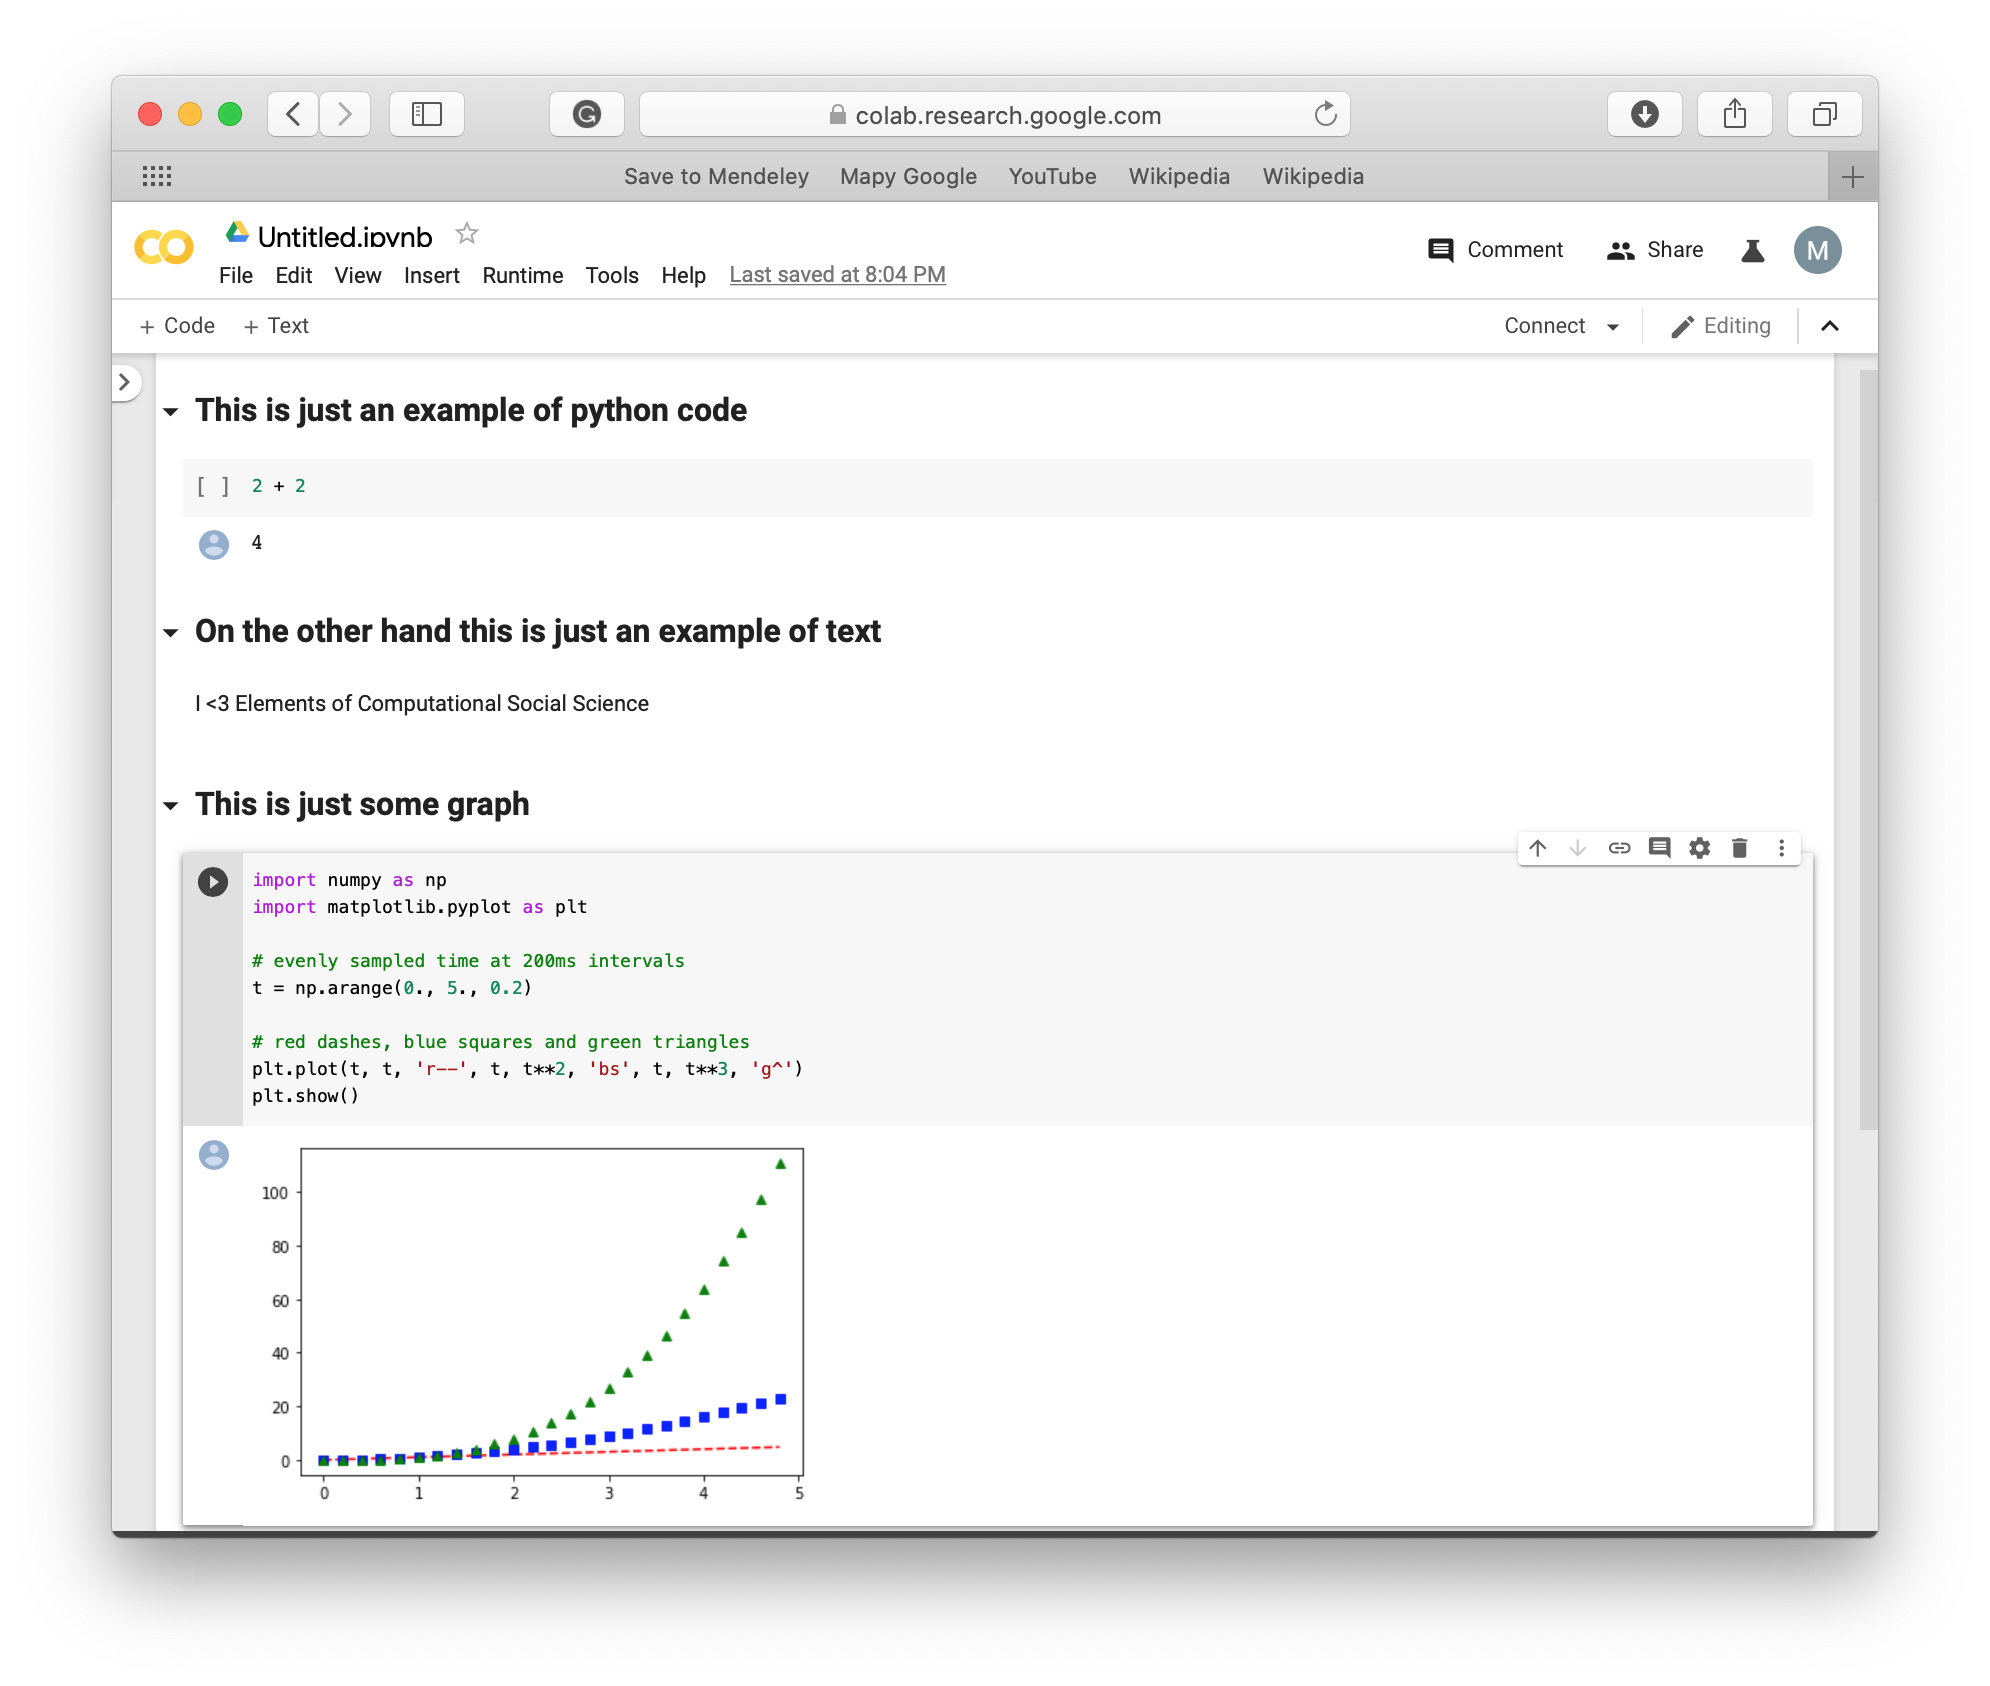
\includegraphics[width = \framewidth]{png/colaboratory.png}
    }
    \only<+>{
        \frametitle{How to open Jupyter Notebook in Colaboratory?}
        If you have a google account and all of you have you just need to follow these four easy steps to open a notebook we prepared for today:
        \begin{enumerate}
            \item Visit \textcolor{blue}{\href{https://colab.research.google.com/notebooks/welcome.ipynb}{www.colab.research.google.com}}
            \item Press File and choose Open notebook\dots
            \item Choose GitHub and type \mintinline{bash}{MikoBie}
            \item Click on \mintinline{bash}{notebooks/N1.ipynb}
        \end{enumerate}
    }
    \only<+>{
        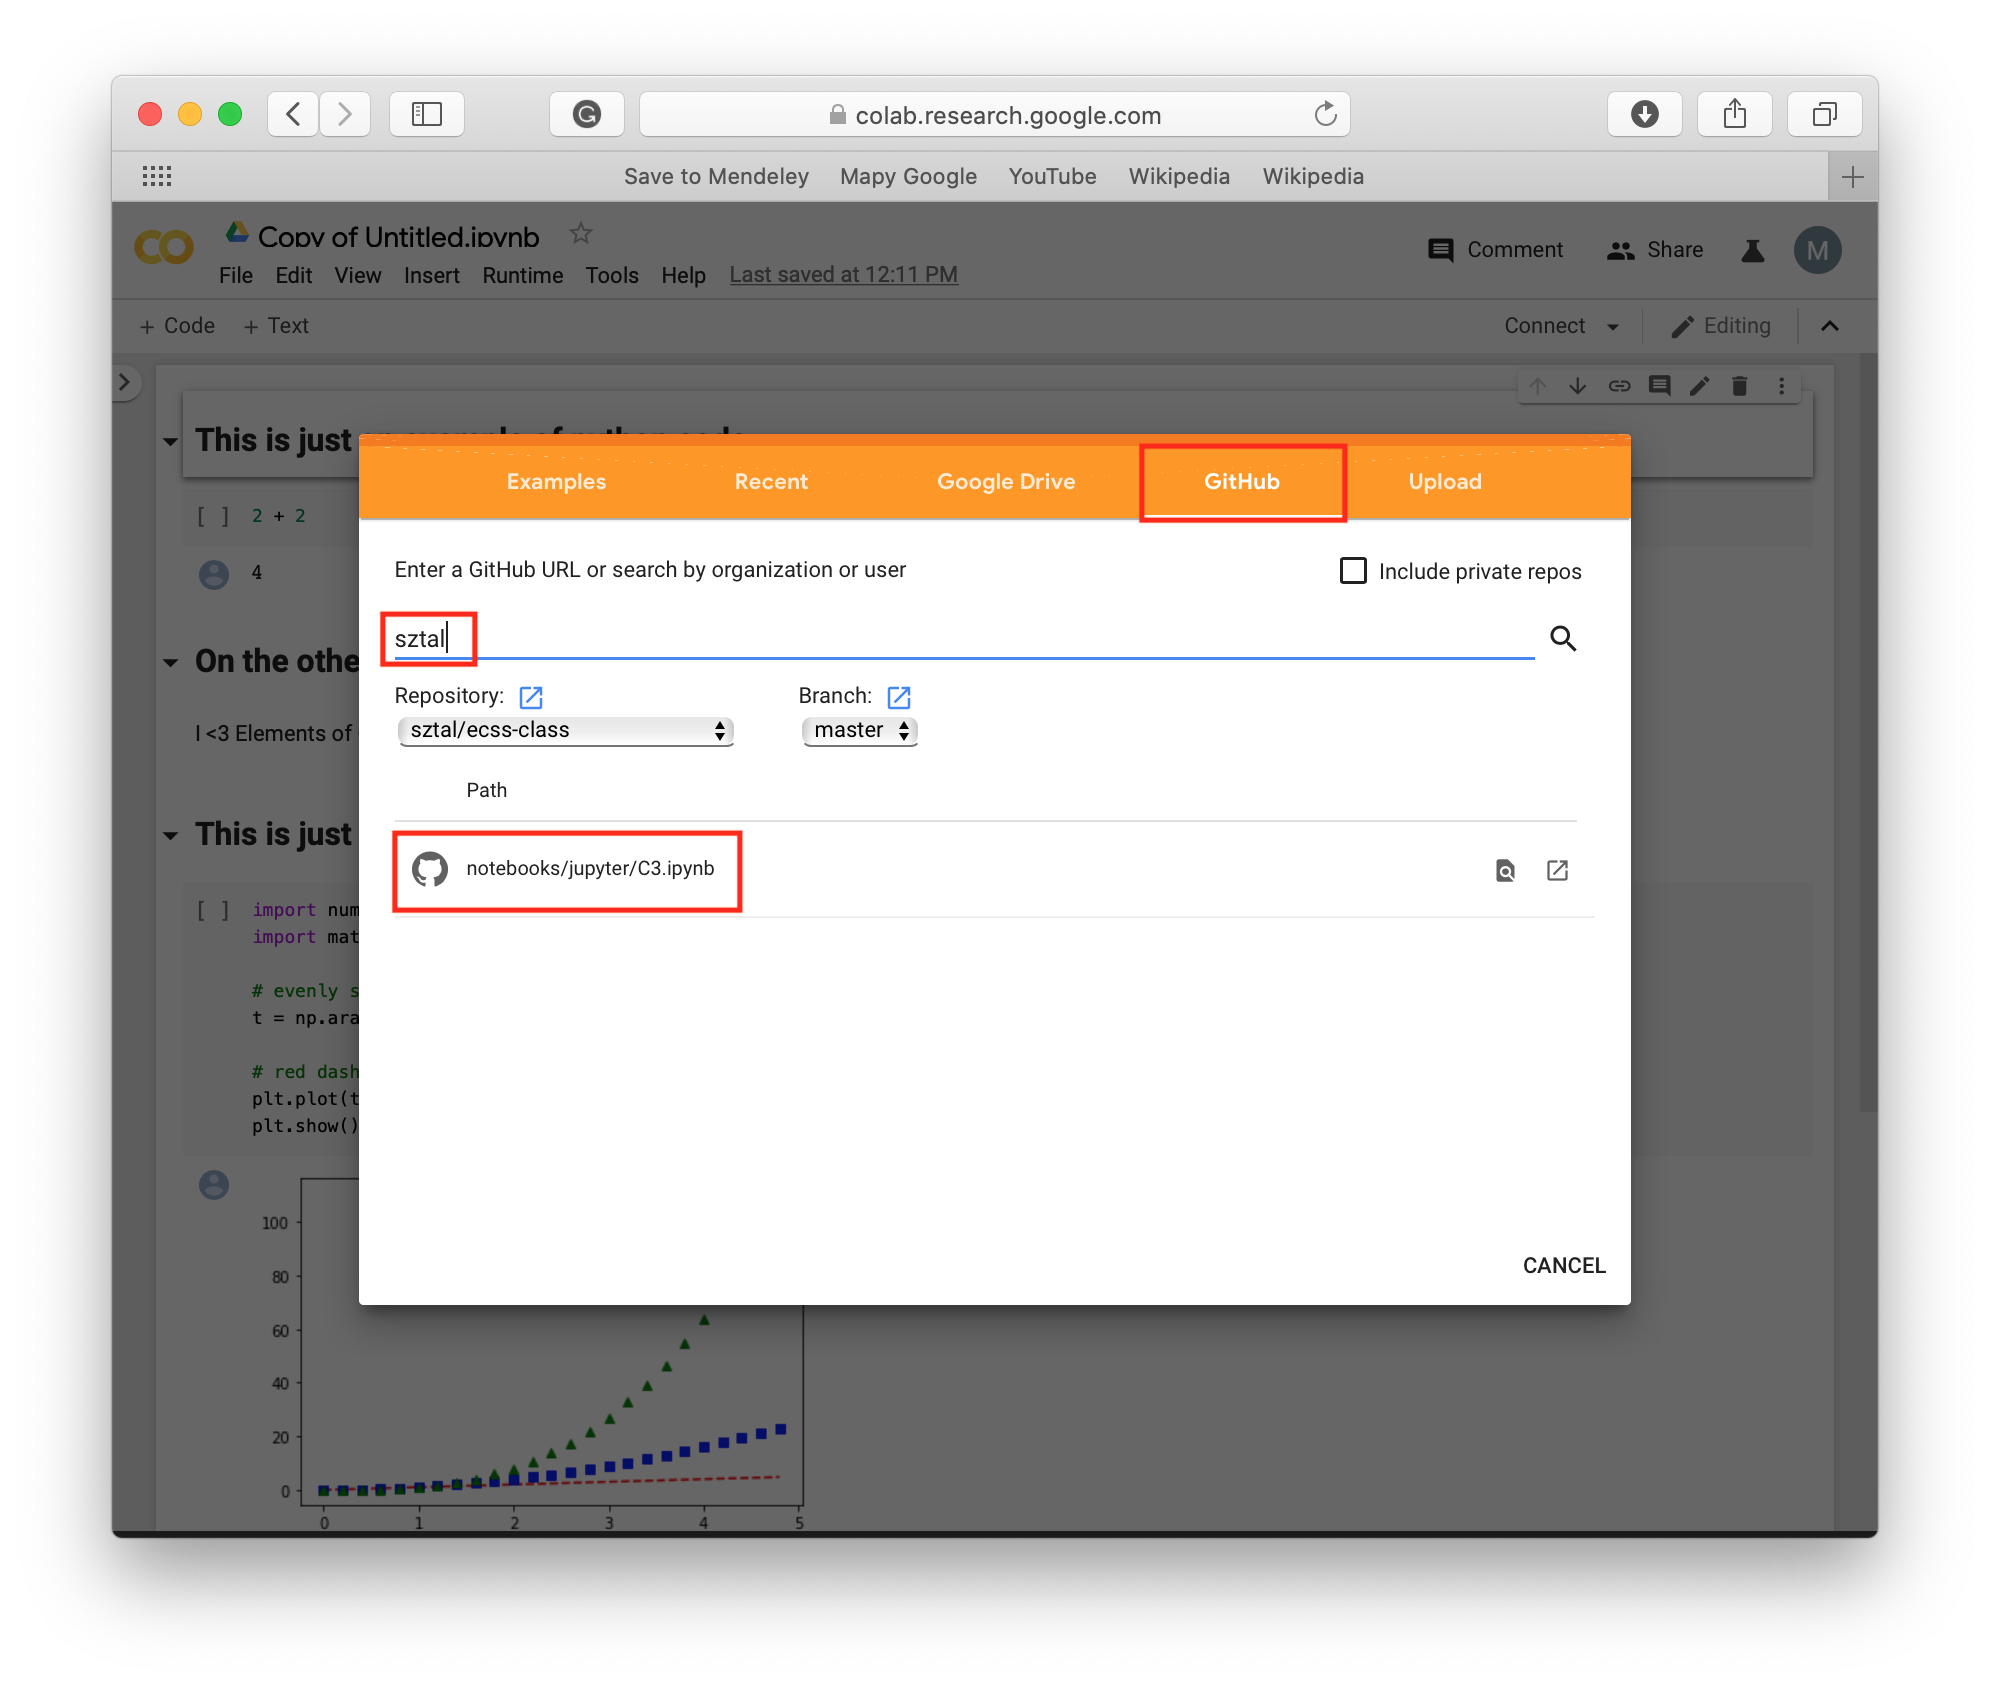
\includegraphics[width = \framewidth]{png/colab_notebook.png}
    }
\end{frame}


\end{document}